% ============================================================
%  Arithmetic Coding and Range Coding
%  Chapter for Data Compression Lecture Notes
%  Dr. Faisal Aslam
% ============================================================

\section{Arithmetic Coding and Range Coding}

\subsection{Introduction}

Entropy coding is the final stage in many compression systems.
Instead of assigning fixed codewords to symbols (like Huffman coding),
\textbf{Arithmetic Coding} and \textbf{Range Coding} represent the entire
message as a single number inside the unit interval $[0,1)$.
This allows code lengths to approach the theoretical entropy limit.

\begin{importantbox}
\textbf{Key Idea.} Arithmetic coding does not assign codes to symbols
individually. Instead, it assigns a code to the entire \emph{sequence} by
repeatedly shrinking an interval. The more probable the message, the larger
the final interval and the fewer bits needed.
\end{importantbox}

% -----------------------------------------------------------
\subsection{Arithmetic Coding: Theory and Algorithm}
% -----------------------------------------------------------

Arithmetic coding encodes a message by repeatedly narrowing an interval in
$[0,1)$. Each symbol reduces the interval based on its probability.

\begin{definitionbox}
\textbf{Algorithm: Arithmetic Coding Encoding.}

\textbf{Step 0 — Initialisation.}
Set $\mathrm{low} = 0$ and $\mathrm{high} = 1$.

\medskip
\textbf{Step 1 — Compute cumulative probabilities.}
Given alphabet $\{s_1, s_2, \ldots, s_k\}$ with probabilities $p(s_i)$,
compute:
\[
  C(s_1) = 0, \qquad C(s_i) = \sum_{j < i} p(s_j), \quad i = 2, 3, \ldots, k.
\]

\textbf{Step 2 — Encode each symbol.}
For each symbol $s$ in the message:
\begin{align*}
  \mathrm{range} &= \mathrm{high} - \mathrm{low} \\
  \mathrm{high}  &= \mathrm{low} + \mathrm{range} \times \bigl(C(s) + p(s)\bigr) \\
  \mathrm{low}   &= \mathrm{low} + \mathrm{range} \times C(s)
\end{align*}

\textbf{Step 3 — Generate the final code.}
After encoding all symbols, output any number $x \in [\mathrm{low},
\mathrm{high})$. Typically the midpoint is used:
\[
  \mathrm{code} = \frac{\mathrm{low} + \mathrm{high}}{2}.
\]
\end{definitionbox}

% -----------------------------------------------------------
\subsection{Example: Arithmetic Coding Step-by-Step}
% -----------------------------------------------------------

\begin{examplebox}
\textbf{Setup.} Alphabet $\{A, B, C\}$ with frequencies $f(A)=5$,
$f(B)=3$, $f(C)=2$, total $= 10$.

\[
  p(A) = 0.5, \qquad p(B) = 0.3, \qquad p(C) = 0.2.
\]

Encode the message $\texttt{BAC}$.

\medskip
\textbf{Step 0 — Initialisation.}
$\mathrm{low} = 0$, $\mathrm{high} = 1$.

\medskip
\textbf{Step 1 — Cumulative probabilities.}
\[
  C(A) = 0, \qquad C(B) = 0.5, \qquad C(C) = 0.8.
\]

\medskip
\textbf{Step 2a — Encode \texttt{B}:}
\begin{align*}
  \mathrm{range} &= 1 - 0 = 1 \\
  \mathrm{high}  &= 0 + 1 \times (0.5 + 0.3) = 0.8 \\
  \mathrm{low}   &= 0 + 1 \times 0.5 = 0.5
\end{align*}
Interval: $[0.5,\ 0.8)$.

\medskip
\textbf{Step 2b — Encode \texttt{A}:}
\begin{align*}
  \mathrm{range} &= 0.8 - 0.5 = 0.3 \\
  \mathrm{high}  &= 0.5 + 0.3 \times (0 + 0.5) = 0.65 \\
  \mathrm{low}   &= 0.5 + 0.3 \times 0 = 0.5
\end{align*}
Interval: $[0.5,\ 0.65)$.

\medskip
\textbf{Step 2c — Encode \texttt{C}:}
\begin{align*}
  \mathrm{range} &= 0.65 - 0.5 = 0.15 \\
  \mathrm{high}  &= 0.5 + 0.15 \times (0.8 + 0.2) = 0.65 \\
  \mathrm{low}   &= 0.5 + 0.15 \times 0.8 = 0.62
\end{align*}
Final interval: $[0.62,\ 0.65)$.

\medskip
\textbf{Step 3 — Final code.}
\[
  \mathrm{code} = \frac{0.62 + 0.65}{2} = 0.635
\]

The value $0.635$ is the arithmetic-coded representation of \texttt{BAC}.
In practice this number would be written out in binary.
\end{examplebox}

\begin{figure}[H]
\centering
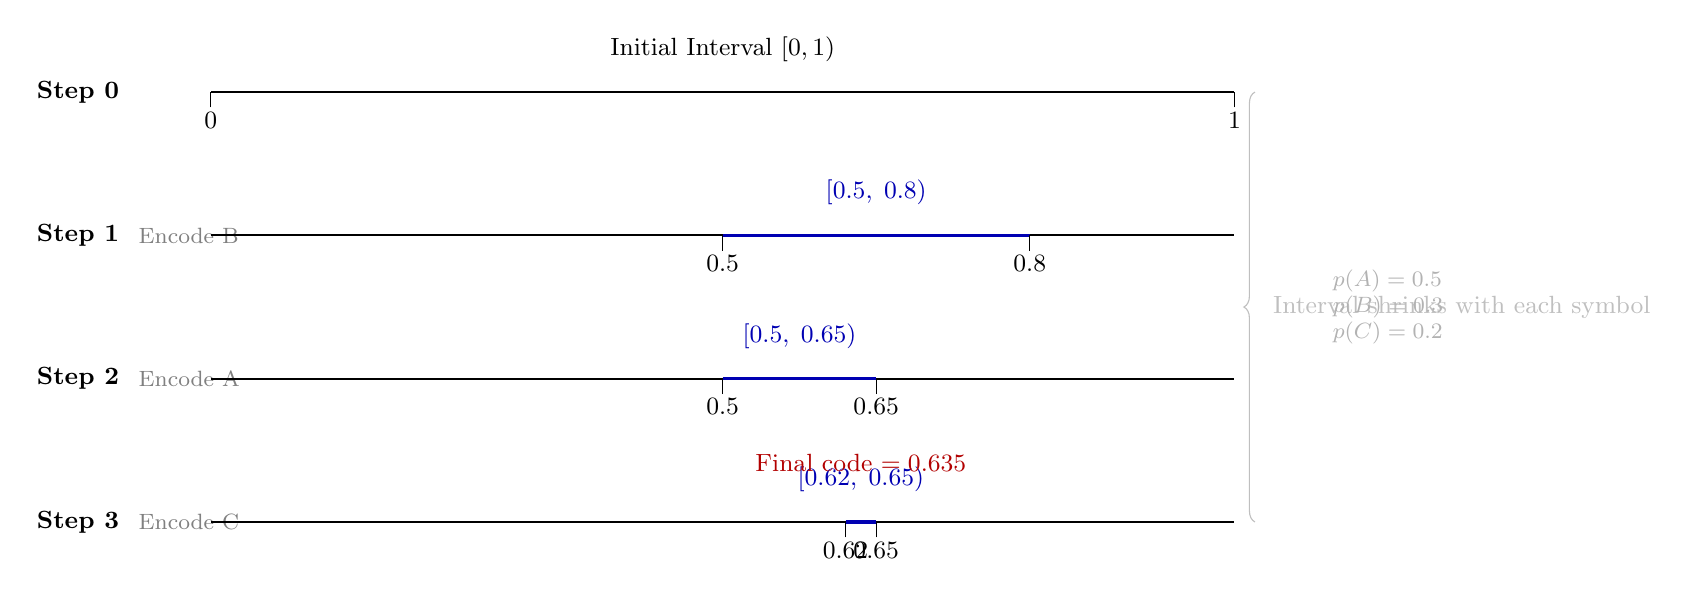
\begin{tikzpicture}[scale=1.3,
    every node/.style={font=\small},
    interval/.style={thick},
    selected/.style={very thick, blue!70!black},
    annotation/.style={font=\footnotesize, text=gray}
]
% Initial interval
\node[anchor=east] at (-0.8,0) {\textbf{Step 0}};
\draw[interval] (0,0) -- (10,0);
\draw[annotation] (0,-0.15) -- (0,0);
\draw[annotation] (10,-0.15) -- (10,0);
\node[below] at (0,-0.1) {$0$};
\node[below] at (10,-0.1) {$1$};
\node[above] at (5,0.2) {Initial Interval $[0,1)$};

% Step 1: Encode B → [0.5, 0.8)
\node[anchor=east] at (-0.8,-1.4) {\textbf{Step 1}};
\node[annotation, right] at (-0.8,-1.4) {Encode B};
\draw[interval] (0,-1.4) -- (10,-1.4);
\draw[selected] (5,-1.4) -- (8,-1.4);
\draw[annotation] (5,-1.55) -- (5,-1.4);
\draw[annotation] (8,-1.55) -- (8,-1.4);
\node[below] at (5,-1.5) {$0.5$};
\node[below] at (8,-1.5) {$0.8$};
\node[above, blue!70!black] at (6.5,-1.2) {$[0.5,\;0.8)$};

% Step 2: Encode A → [0.5, 0.65)
\node[anchor=east] at (-0.8,-2.8) {\textbf{Step 2}};
\node[annotation, right] at (-0.8,-2.8) {Encode A};
\draw[interval] (0,-2.8) -- (10,-2.8);
\draw[selected] (5,-2.8) -- (6.5,-2.8);
\draw[annotation] (5,-2.95) -- (5,-2.8);
\draw[annotation] (6.5,-2.95) -- (6.5,-2.8);
\node[below] at (5,-2.9) {$0.5$};
\node[below] at (6.5,-2.9) {$0.65$};
\node[above, blue!70!black] at (5.75,-2.6) {$[0.5,\;0.65)$};

% Step 3: Encode C → [0.62, 0.65)
\node[anchor=east] at (-0.8,-4.2) {\textbf{Step 3}};
\node[annotation, right] at (-0.8,-4.2) {Encode C};
\draw[interval] (0,-4.2) -- (10,-4.2);
\draw[selected] (6.2,-4.2) -- (6.5,-4.2);
\draw[annotation] (6.2,-4.35) -- (6.2,-4.2);
\draw[annotation] (6.5,-4.35) -- (6.5,-4.2);
\node[below] at (6.2,-4.3) {$0.62$};
\node[below] at (6.5,-4.3) {$0.65$};
\node[above, blue!70!black] at (6.35,-4.0) {$[0.62,\;0.65)$};
\node[above, red!70!black] at (6.35,-3.8) {Final code $= 0.635$};

\draw[decorate, decoration={brace, amplitude=4pt, mirror}, gray!50]
    (10.2,0) -- (10.2,-4.2) node[midway, right, xshift=3pt]
    {Interval shrinks with each symbol};
\node[annotation, text=gray!60, align=left] at (11.5,-2.1)
    {$p(A)=0.5$\\ $p(B)=0.3$\\ $p(C)=0.2$};
\end{tikzpicture}
\caption{Arithmetic Coding interval refinement for message \texttt{BAC}.
Each step selects a sub-interval based on the symbol being encoded.
The final code $0.635$ is the midpoint of $[0.62, 0.65)$.}
\label{fig:arithmetic}
\end{figure}

% -----------------------------------------------------------
\subsection{Why People Prefer Range Coding}
% -----------------------------------------------------------

Arithmetic coding is theoretically elegant but has practical implementation
challenges:

\begin{itemize}[leftmargin=2em]
    \item \textbf{Arbitrary precision requirement.} As encoding progresses the
          interval becomes very small, requiring high-precision or
          arbitrary-precision arithmetic for long messages.
    \item \textbf{Incremental output complexity.} Outputting bits
          incrementally (before the whole message is encoded) requires careful
          handling of carry propagation — a process called
          \emph{normalisation} or \emph{bit-stuffing}.
    \item \textbf{Computational cost.} Floating-point multiplications and
          divisions at each step are more expensive than the integer operations
          used in range coding.
    \item \textbf{Historical patent issues.} Arithmetic coding was subject to
          patents for many years, discouraging its use in some applications
          (though this is no longer an issue today).
\end{itemize}

\begin{importantbox}
\textbf{Normalisation in Arithmetic Coding.}
The term \emph{normalisation} in arithmetic coding refers to
\textbf{outputting bits incrementally} as they become known — not to
preventing precision loss.  For example, once the interval lies entirely
within $[0.5, 1)$, the first output bit must be \texttt{1} and can be
emitted immediately. The interval is then doubled and encoding continues.

If we are content to store the entire final fraction (like $0.635$) without
incremental output, no normalisation is needed; but for long messages storing
the full-precision fraction is impractical.
\end{importantbox}

\textbf{Range Coding} addresses these challenges by using fixed-precision
integer arithmetic (e.g.\ 32-bit or 64-bit integers), handling incremental
output through renormalisation, and using only integer operations (division,
multiplication, shifts). Range coding is simply a
\textbf{reparameterisation of arithmetic coding} designed for efficient
implementation.

% -----------------------------------------------------------
\subsection{Range Coding: Theory and Algorithm}
% -----------------------------------------------------------

Range coding works on integers rather than real-number intervals. The
fundamental insight is to scale the $[0,1)$ interval to a large integer range
$[0, 2^{32})$; all operations then become integer arithmetic.

\begin{definitionbox}
\textbf{Algorithm: Range Coding Encoding.}

\textbf{Step 0 — Initialisation.}
Set $\mathrm{low} = 0$ and $\mathrm{range} = R$ (a large integer, typically
$2^{32}$).

\medskip
\textbf{Step 1 — Compute cumulative frequencies.}
Given alphabet $\{s_1, \ldots, s_k\}$ with integer frequencies $f(s_i)$ and
$\mathrm{total} = \sum_i f(s_i)$, compute:
\[
  C(s_1) = 0, \qquad C(s_i) = \sum_{j < i} f(s_j), \quad i = 2, \ldots, k.
\]

\textbf{Step 2 — Encode each symbol.}
For each symbol $s$:
\begin{enumerate}[leftmargin=2em]
    \item $\mathrm{unit} = \lfloor \mathrm{range} / \mathrm{total} \rfloor$
    \item $\mathrm{low} \mathrel{+}= \mathrm{unit} \times C(s)$
    \item $\mathrm{range} = \mathrm{unit} \times f(s)$
    \item \textbf{Renormalisation:} while $\mathrm{range} < 2^{24}$, output
          the top byte of $\mathrm{low}$ and shift both $\mathrm{low}$ and
          $\mathrm{range}$ left by 8 bits.
\end{enumerate}

\textbf{Step 3 — Flush.}
Output the remaining bytes of $\mathrm{low}$.
\end{definitionbox}

% -----------------------------------------------------------
\subsection{Range Coding Example: Message \texttt{BAC}}
% -----------------------------------------------------------

\begin{examplebox}
We encode \texttt{BAC} using integer range coding with $R = 2^{16} = 65536$
for readability (the process is identical with $2^{32}$).

\medskip
\textbf{Cumulative frequencies:}
$f(A)=5,\ f(B)=3,\ f(C)=2$, total $=10$.
$C(A)=0,\ C(B)=5,\ C(C)=8$.

\medskip
\textbf{Symbol 1 — \texttt{B}:}
\begin{align*}
  \mathrm{unit} &= \lfloor 65536 / 10 \rfloor = 6553 \\
  \mathrm{low}  &= 0 + 6553 \times 5 = 32765 \\
  \mathrm{range}&= 6553 \times 3 = 19659
\end{align*}
Real-number equivalent: $\approx [0.5000,\ 0.8000)$.

\medskip
\textbf{Symbol 2 — \texttt{A}:}
\begin{align*}
  \mathrm{unit} &= \lfloor 19659 / 10 \rfloor = 1965 \\
  \mathrm{low}  &= 32765 + 1965 \times 0 = 32765 \\
  \mathrm{range}&= 1965 \times 5 = 9825
\end{align*}
Real-number equivalent: $\approx [0.5000,\ 0.6500)$.

\medskip
\textbf{Symbol 3 — \texttt{C}:}
\begin{align*}
  \mathrm{unit} &= \lfloor 9825 / 10 \rfloor = 982 \\
  \mathrm{low}  &= 32765 + 982 \times 8 = 40621 \\
  \mathrm{range}&= 982 \times 2 = 1964
\end{align*}
Real-number equivalent: $\approx [0.6198,\ 0.6498)$.

\medskip
No renormalisation is triggered for this short message. Final integer interval:
$[40621,\ 42585)$. We output $\mathrm{low} = 40621$.
\end{examplebox}

\begin{figure}[H]
\centering
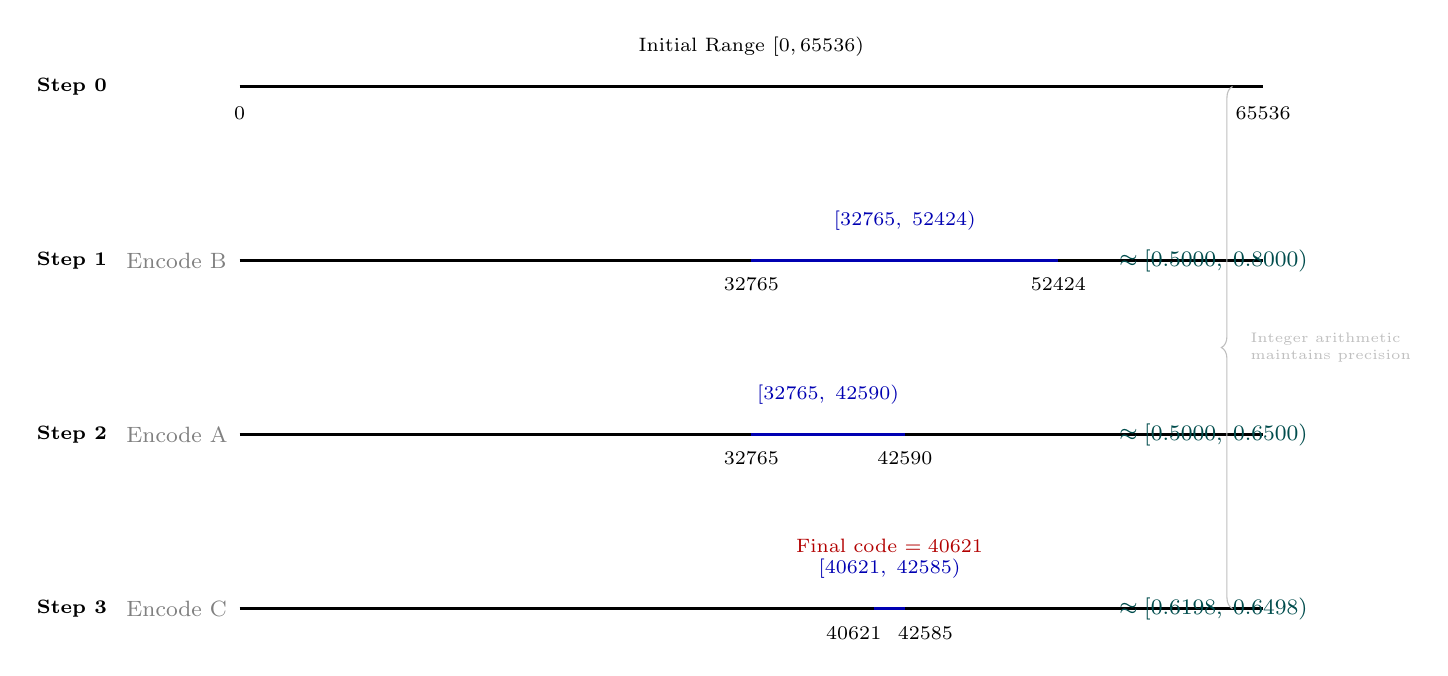
\begin{tikzpicture}[scale=1.3,
    every node/.style={font=\scriptsize},
    interval/.style={thick},
    selected/.style={very thick, blue!70!black},
    annotation/.style={font=\footnotesize, text=gray}
]
\def\stepheight{1.7}

\node[anchor=east] at (-1.2,0) {\textbf{Step 0}};
\draw[interval] (0,0) -- (10,0);
\node[below] at (0,-0.1) {$0$};
\node[below] at (10,-0.1) {$65536$};
\node[above] at (5,0.2) {Initial Range $[0,65536)$};

\node[anchor=east] at (-1.2,-\stepheight) {\textbf{Step 1}};
\node[annotation, right] at (-1.2,-\stepheight) {Encode B};
\draw[interval] (0,-\stepheight) -- (10,-\stepheight);
\draw[selected] (5,-\stepheight) -- (8,-\stepheight);
\node[below] at (5,-\stepheight-0.08) {$32765$};
\node[below] at (8,-\stepheight-0.08) {$52424$};
\node[above, blue!70!black] at (6.5,-\stepheight+0.2) {$[32765,\;52424)$};
\node[annotation, text=teal!60!black, anchor=west] at (8.5,-\stepheight)
    {$\approx [0.5000,\;0.8000)$};

\node[anchor=east] at (-1.2,-2*\stepheight) {\textbf{Step 2}};
\node[annotation, right] at (-1.2,-2*\stepheight) {Encode A};
\draw[interval] (0,-2*\stepheight) -- (10,-2*\stepheight);
\draw[selected] (5,-2*\stepheight) -- (6.5,-2*\stepheight);
\node[below] at (5,-2*\stepheight-0.08) {$32765$};
\node[below] at (6.5,-2*\stepheight-0.08) {$42590$};
\node[above, blue!70!black] at (5.75,-2*\stepheight+0.2) {$[32765,\;42590)$};
\node[annotation, text=teal!60!black, anchor=west] at (8.5,-2*\stepheight)
    {$\approx [0.5000,\;0.6500)$};

\node[anchor=east] at (-1.2,-3*\stepheight) {\textbf{Step 3}};
\node[annotation, right] at (-1.2,-3*\stepheight) {Encode C};
\draw[interval] (0,-3*\stepheight) -- (10,-3*\stepheight);
\draw[selected] (6.2,-3*\stepheight) -- (6.5,-3*\stepheight);
\node[below] at (6.0,-3*\stepheight-0.08) {$40621$};
\node[below] at (6.7,-3*\stepheight-0.08) {$42585$};
\node[above, blue!70!black] at (6.35,-3*\stepheight+0.2) {$[40621,\;42585)$};
\node[above, red!70!black] at (6.35,-3*\stepheight+0.45) {Final code $=40621$};
\node[annotation, text=teal!60!black, anchor=west] at (8.5,-3*\stepheight)
    {$\approx [0.6198,\;0.6498)$};

\draw[decorate, decoration={brace, amplitude=4pt, mirror}, gray!50]
    (9.7,0) -- (9.7,-3*\stepheight) node[midway, right, xshift=3pt, align=left, font=\tiny]
    {Integer arithmetic\\ maintains precision};
\end{tikzpicture}
\caption{Range Coding integer-interval refinement for message \texttt{BAC}.
Real-number equivalents are shown to the right.}
\label{fig:range}
\end{figure}

% -----------------------------------------------------------
\subsection{Range Coding with Renormalisation}
% -----------------------------------------------------------

The previous example was short enough that the range never shrank below the
renormalisation threshold. We now encode a longer message to see renormalisation
in action.

\begin{examplebox}
\textbf{Encode \texttt{B A C C C C} with $R = 2^{32}$.}

Same alphabet: $f(A)=5,\ f(B)=3,\ f(C)=2$, total $=10$.
$C(A)=0,\ C(B)=5,\ C(C)=8$.

\medskip
\begin{center}
\rowcolors{2}{blue!5}{white}
\begin{tabular}{@{}clrrl@{}}
\toprule
\textbf{Step} & \textbf{Symbol} & \textbf{low} & \textbf{range} & \textbf{Output} \\
\midrule
0 & — & $0$ & $4{,}294{,}967{,}296$ & — \\
1 & B & $2{,}147{,}483{,}645$ & $1{,}288{,}490{,}187$ & — \\
2 & A & $2{,}147{,}483{,}645$ & $644{,}245{,}090$ & — \\
3 & C & $2{,}662{,}879{,}717$ & $128{,}849{,}018$ & — \\
4 & C & $2{,}765{,}958{,}925$ & $25{,}769{,}802$ & — \\
5 & C & $2{,}786{,}574{,}765$ & $5{,}153{,}960$ & \textbf{Renorm!} \\
Renorm & — & $439{,}463{,}680$ & $1{,}319{,}413{,}760$ & \texttt{0xA6} (166) \\
6 & C & $1{,}494{,}994{,}688$ & $263{,}882{,}752$ & — \\
\bottomrule
\end{tabular}
\end{center}

\medskip
\textbf{Why does renormalisation trigger after symbol 5?}
Each $C$ shrinks the range by a factor of $\approx 0.2$:
\[
  644{,}245{,}090 \xrightarrow{\times 0.2} 128{,}849{,}018
  \xrightarrow{\times 0.2} 25{,}769{,}802
  \xrightarrow{\times 0.2} 5{,}153{,}960 < 2^{24}.
\]

\textbf{Renormalisation step:} output the top byte of $\mathrm{low}$
($2{,}786{,}574{,}765 \gg 24 = 166 = \texttt{0xA6}$), then shift both
$\mathrm{low}$ and $\mathrm{range}$ left by 8 bits.

\medskip
\textbf{Final output stream:}
$[\texttt{0xA6},\ \texttt{0x59},\ \texttt{0x1C},\ \texttt{0x00},\ \texttt{0x00}]$
(the renorm byte followed by the four bytes of the final $\mathrm{low}$).
\end{examplebox}

% -----------------------------------------------------------
\subsection{Range Coding: Decoding Algorithm}
% -----------------------------------------------------------

Decoding is the exact inverse of encoding. Given the compressed stream we
reconstruct the original symbols by determining which symbol's interval
contains the current code value.

\begin{definitionbox}
\textbf{Algorithm: Range Coding Decoding.}

\textbf{Step 0 — Initialisation.}
Set $\mathrm{low} = 0$, $\mathrm{range} = R$.  Read the first 4 bytes of the
stream to form the initial $\mathrm{code}$.

\medskip
\textbf{Step 1 — Cumulative frequencies} — same as encoder.

\medskip
\textbf{Step 2 — Decode each symbol.}
For each symbol position:
\begin{enumerate}[leftmargin=2em]
    \item $\mathrm{unit} = \lfloor \mathrm{range} / \mathrm{total} \rfloor$
    \item Find symbol $s$ satisfying:
    \[
      C(s) \;\leq\; \frac{\mathrm{code} - \mathrm{low}}{\mathrm{unit}} 
      \;<\; C(s) + f(s)
    \]
    \item Output symbol $s$.
    \item $\mathrm{low} \mathrel{+}= \mathrm{unit} \times C(s)$; \quad
          $\mathrm{range} = \mathrm{unit} \times f(s)$.
    \item \textbf{Renormalisation:} while $\mathrm{range} < 2^{24}$:
    \begin{align*}
      \mathrm{low}  &\leftarrow (\mathrm{low} \ll 8)\ \&\ (2^{32}-1) \\
      \mathrm{code} &\leftarrow \bigl((\mathrm{code} \ll 8)\ \&\ 
                     (2^{32}-1)\bigr) \mid \mathrm{next\_byte} \\
      \mathrm{range}&\leftarrow \mathrm{range} \ll 8
    \end{align*}
\end{enumerate}
\end{definitionbox}

\begin{importantbox}
\textbf{Encoder–Decoder Symmetry.}
Both sides shift $\mathrm{low}$ and $\mathrm{range}$ left by 8 bits during
renormalisation. The encoder \emph{outputs} the byte that falls off the top of
$\mathrm{low}$; the decoder \emph{reads} that same byte and inserts it at the
bottom of $\mathrm{code}$.  This is why the decoder maintains a separate
$\mathrm{code}$ variable — it tracks the ``window'' into the compressed
stream.
\end{importantbox}

% -----------------------------------------------------------
\subsection{Decoding Example: Recovering \texttt{B A C C C C}}
% -----------------------------------------------------------

\begin{examplebox}
\textbf{Input stream:}
$[\texttt{0xA6},\ \texttt{0x59},\ \texttt{0x1C},\ \texttt{0x00},
\ \texttt{0x00}]$.

Initialise: $\mathrm{low}=0$, $\mathrm{range}=2^{32}$,
$\mathrm{code} = \texttt{0xA6591C00} = 2{,}789{,}021{,}696$.

\medskip
\begin{center}
\rowcolors{2}{green!5}{white}
\begin{tabular}{@{}crrrr@{}}
\toprule
\textbf{Step} & \textbf{code} & \textbf{low} & \textbf{range} 
              & \textbf{Symbol} \\
\midrule
Start  & $2{,}789{,}021{,}696$ & $0$ & $4{,}294{,}967{,}296$ & — \\
1 & $2{,}789{,}021{,}696$ & $2{,}147{,}483{,}645$ & $1{,}288{,}490{,}187$ & B \\
2 & $2{,}789{,}021{,}696$ & $2{,}147{,}483{,}645$ & $644{,}245{,}090$ & A \\
3 & $2{,}789{,}021{,}696$ & $2{,}662{,}879{,}717$ & $128{,}849{,}018$ & C \\
4 & $2{,}789{,}021{,}696$ & $2{,}765{,}958{,}925$ & $25{,}769{,}802$ & C \\
5 & $2{,}789{,}021{,}696$ & $2{,}786{,}574{,}765$ & $5{,}153{,}960$ & C \\
Renorm & $1{,}494{,}994{,}688$ & $439{,}463{,}680$ & $1{,}319{,}413{,}760$ & — \\
6 & $1{,}494{,}994{,}688$ & $439{,}463{,}680$ & $1{,}319{,}413{,}760$ & C \\
\bottomrule
\end{tabular}
\end{center}

\medskip
\textbf{Sample decode step (Symbol 1):}
\[
  \frac{\mathrm{code} - \mathrm{low}}{\mathrm{unit}} 
  = \frac{2{,}789{,}021{,}696}{429{,}496{,}729} \approx 6.49
\]
Since $C(B) = 5 \leq 6.49 < 8 = C(B)+f(B)$, decoded symbol $= B$. \checkmark

\medskip
\textbf{Renormalisation (after Symbol 5):}
Read next byte \texttt{0x00} from stream.
\begin{align*}
  \mathrm{code} &\leftarrow \texttt{0xA6591C00} \ll 8 \mid \texttt{0x00}
                 = \texttt{0x591C0000} = 1{,}494{,}994{,}688 \\
  \mathrm{low}  &\leftarrow \texttt{0xA61A2FAD} \ll 8 
                 = \texttt{0x1A2FAD00} = 439{,}463{,}680 \\
  \mathrm{range}&\leftarrow 5{,}153{,}960 \times 256 = 1{,}319{,}413{,}760
\end{align*}

Recovered sequence: $\boxed{\texttt{B\ A\ C\ C\ C\ C}}$. \checkmark
\end{examplebox}

% -----------------------------------------------------------
\subsection{Arithmetic vs.\ Range Coding: A Comparison}
% -----------------------------------------------------------

\begin{center}
\rowcolors{2}{blue!6}{white}
\begin{tabular}{@{}p{3.8cm}p{4.8cm}p{4.8cm}@{}}
\toprule
\textbf{Concept} & \textbf{Arithmetic Coding} & \textbf{Range Coding} \\
\midrule
Representation & Real numbers in $[0,1)$ & Integers in $[0, R)$ \\
Initial state & $\mathrm{low}=0$, $\mathrm{high}=1$ & $\mathrm{low}=0$, $\mathrm{range}=R$ \\
Unit size & $\mathrm{high} - \mathrm{low}$ & $\lfloor\mathrm{range}/\mathrm{total}\rfloor$ \\
Low update & $\mathrm{low} + \mathrm{range} \times C(s)$ & $\mathrm{low} + \mathrm{unit} \times C(s)$ \\
Range update & $\mathrm{range} \times p(s)$ & $\mathrm{unit} \times f(s)$ \\
Precision & Floating-point normalisation & Integer renormalisation \\
Final code & Midpoint of final interval & Value from final interval \\
Arithmetic & Float multiply/divide & Integer multiply/divide \\
Speed & Moderate & Fast \\
\bottomrule
\end{tabular}
\end{center}

The two methods are mathematically equivalent; range coding is an
integer-based reparameterisation of arithmetic coding.

% -----------------------------------------------------------
\subsection{Summary}
% -----------------------------------------------------------

\begin{itemize}[leftmargin=2em]
    \item Arithmetic coding uses real-number intervals and is mathematically 
          elegant but requires floating-point or arbitrary-precision arithmetic.
    \item Range coding uses integer intervals and produces the same compressed
          result using only fast integer operations.
    \item Both achieve compression close to the theoretical Shannon entropy 
          limit.
    \item \emph{Renormalisation} in range coding outputs bytes incrementally 
          as the range shrinks below $2^{24}$, keeping the state in a 
          fixed-width integer register.
    \item Decoding mirrors encoding exactly: the decoder maintains a 
          $\mathrm{code}$ variable that tracks the current position in the 
          compressed stream and updates $\mathrm{low}$ and $\mathrm{range}$ 
          identically to the encoder.
    \item During renormalisation the encoder outputs the byte that falls off 
          the top of $\mathrm{low}$; the decoder reads that byte and inserts 
          it at the bottom of $\mathrm{code}$.
\end{itemize}

% -----------------------------------------------------------
\subsection{Exercises}
% -----------------------------------------------------------

\begin{exercisebox}
Encode the message \texttt{CAB} using arithmetic coding with $p(A)=0.5$,
$p(B)=0.3$, $p(C)=0.2$.  Show the interval after each symbol and state the
final code.
\end{exercisebox}

\begin{exercisebox}
Encode the same message \texttt{CAB} using range coding with $R=65536$ and
the same frequencies.  Compare the final integer interval with the
real-number interval from the previous exercise.
\end{exercisebox}

\begin{exercisebox}
Explain in your own words why range coding is more suitable for hardware
implementation than arithmetic coding.  Give at least two concrete reasons.
\end{exercisebox}

\begin{exercisebox}
What would happen if we used a very small initial range such as $R=100$ for
range coding?  How would the integer truncation in
$\mathrm{unit} = \lfloor \mathrm{range}/\mathrm{total} \rfloor$ affect
compression quality?
\end{exercisebox}

\begin{exercisebox}
Write pseudocode for an arithmetic coding encoder and a range coding encoder
side-by-side.  Highlight the three lines that differ between the two.
\end{exercisebox}

\begin{exercisebox}
Using the renormalisation example (\texttt{B A C C C C}), encode the shorter
message \texttt{B A C C} instead.  Would renormalisation be triggered?
Justify your answer by tracking the range at each step.
\end{exercisebox}

\begin{exercisebox}
\textbf{Decoding practice.}  Using the decoding algorithm, decode the
compressed output you produced in Exercise~\theexercise\  (the \texttt{CAB}
encoding) to verify you recover the original message.  Show the offset
computation at each step.
\end{exercisebox}

\begin{exercisebox}
Explain the encoder–decoder symmetry during renormalisation.  Why does the
decoder shift $\mathrm{code}$ left and insert the next byte, while the
encoder shifts $\mathrm{low}$ left and outputs the falling byte?  What
ensures the two sides stay synchronised?
\end{exercisebox}
